Para simular a concentração na superfície durante nitretação gasosa de acordo com a descrição dada na Seção \autoref{sec:sol-numerica-2alei2}, foram utilizados os paramêtros dados pela \autoref{tab:parametros_csvar}.

\begin{table}[ht]
\centering
\setlength{\doublerulesep}{\arrayrulewidth}
{\def\arraystretch{2}\tabcolsep=10pt
\caption{Parâmetros para concentração na superfície variável nitretação gasosa}
\resizebox{\textwidth}{!}{
\begin{tabular}{c c c}
\hline\hline
Parâmetro & Descrição & Valor \\\hline
$\beta$ & Coeficiente para relacionar velocidade em que se atinge o equilíbrio & 0,0001 \\
$C_{eq}$ & Concentração de equilíbrio entre gás e aço &  47.318,64 mol/m$^3$ (2,0358 $\times$ 10$^{28}$ m$^-3$)    \\
\hline\hline
\end{tabular}
\label{tab:parametros_csvar}
}
}
\end{table}

Os valores da \autoref{tab:parametros_csvar} foram retirados de \cite{christiansen2008nitrogen}. O valor de $\beta$ foi definido testando o melhor \textit{fit} em dados experimentais e $C_{eq}$ foi definido como descrito na seção \autoref{sec:modelo11}.

Os resultados mostrando a concentração de nitrogênio em função da profundidade ao longo do tempo para a simulação com concentração superficial variável estão representados na Figura \ref{fig:csvar-gas}.

\begin{figure}[ht]
\centering
	\caption{Resultado simulação para concentração na superfície variável considerando nitretação a gás, até 2 horas}
	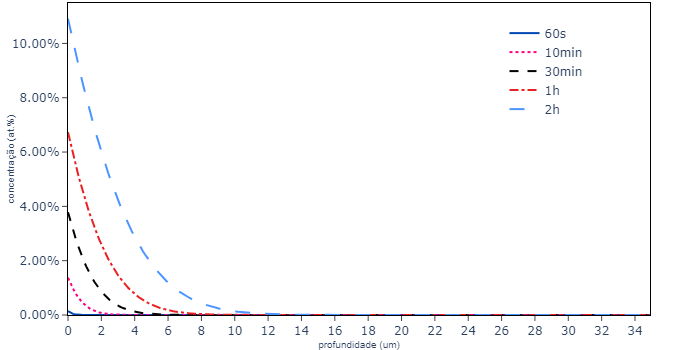
\includegraphics[width=1.0\textwidth]{plot_fickGas}
	\label{fig:csvar-gas}
	\centering
	\fonte{Elaborado pela autora}
\end{figure}

\begin{figure}[ht]
\centering
	\caption{Resultado simulação para concentração na superfície variável considerando nitretação a gás, até 22 horas}
	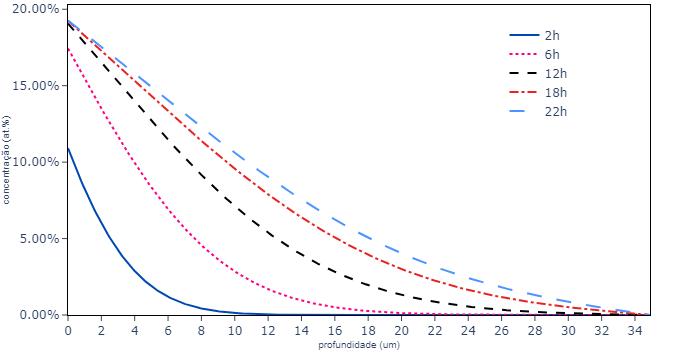
\includegraphics[width=1.0\textwidth]{plot_fickGas2}
	\label{fig:csvar-gas}
	\centering
	\fonte{Elaborado pela autora}
\end{figure}

\myworries{//escrever sobre os gráficos}

\myworries{//adicionar a plasma - para simular a plasma preciso de um j --> OK - arrumar e rodar (PC Lu)}